\chapter{Multifactorial emotion estimation}

In the games research field, there have been studies aiming at using such theory and psychophysiological methods applied to game research \parencite{kivikangas2011review}. It has been demonstrated that it is possible to use physiological signals to automatically assess different emotional states in the context of games using a variety of signals \parencite{bousefsaf2013remote,yun2009game,rani2006empirical,tijs2008dynamic}. The use of a single signal for the assessment is feasible, however a mapping process based on a multimodal analysis, when more than one signal is used, is more likely to produce accurate results \parencite{kukolja2014comparative}. A combination of signals can reduce the interference/noise caused by signal manipulation. Physiological signals, e.g. HR, are considered reliable sources since they are hard to fake (because of their link to the ANS), differently from facial expressions \parencite{Landowska}, for instance. When combined in the same analysis, however, those signals can complement each other and provide more information about emotional states.

The first multimodal analysis approaches were based on obtrusive measurements of the input signals, where physical sensors were used. \textcite{Chanel_2011}, for instance, demonstrated the use of multimodal input analysis to measure emotions and involvement in a game context. Participants played Tetris in different difficulty conditions while being monitored by a variety of sensors, which included a respiration belt and an electroencephalogram (EEG) system. The data from the EEG and the other peripheral signals were computed into two groups of features, which were used to train classifiers to recognize the states: boredom (low pleasure and low pressure, associated with easy difficulty), engagement (higher pleasure and motivation, associated with medium difficulty) and stress (anxiety and low pleasure, associated with hard difficulty). The classification accuracy of the model varied between 48\% and 55\% for different input signals, classifiers and feature selection.

\textcite{grundlehner2009design} also used physical sensors to perform real-time continuous arousal monitoring. Using a wireless sensor network for signal acquisition, the authors record and use four signals from subjects to estimate arousal: electrocardiogram (ECG), respiration, skin conductance and skin temperature. The ECG is used to calculate HRV, which is then used in the estimation. The data used for emotion-triggering was based on videos, sounds and a cognitive demanding game. A regression analysis is performed to identify the importance of the features in the estimation of arousal. $HRV_{LF}$ and $HRV_{HF}$ were not significant when compared to the other signals (e.g. skin conductance), while the standard deviation of HRV presented a significant weight. The arousal prediction matches the hypothesized arousal events marked by the authors in each of the emotion-triggering content. The results, however, were performed with controlled, pre-defined events that are expected to cause reactions, which might be related to arousal. More subtle or dynamic interactions, such as the ones obtained when a subject plays a digital game, might not be identified or detected by the approach proposed by the authors.

\parencite{bailenson2008real} used a combination of physiological signals (obtained from physical sensors) and facial expressions. The authors used a machine learning model to map the input signals to emotions (sadness or amusement). The training data used for the machine learning model was based on recordings of participants while they watched a video containing different emotion-triggering segments (neutral, amusement and sadness). Additionally 15 physiological signals were also used, among them HR, skin conductance level and finger temperature. The video recordings were annotated by professional coders; the annotated video frames were used in conjunction with the physiological signals to produce the predicting model. The authors compared the performance of models built from different data sources, such as the data from all subjects (general model), or from the female/male population (gender-specific model) or from a single individual (person-specific model). The model performed better when categorizing emotions instead of predicting its intensities and when detecting amusement instead of sadness. Additionally the person-specific model outperformed the other two variations, suggesting that a person-tailored model might be more effective in identifying features (even the more subtle ones) than a general-purpose model. The results also state that a model built from a combination of facial and physiological information is more efficient than a model built with either one alone.

\textcite{mental} proposed a completely non-obtrusive and remote approach based on multimodal analysis to identify user emotion. The main goal of such approach is aimed at monitoring patients mental health states. The model was created by weighting different features created from input signals, all obtained unobtrusively from a video of the subject's face and the textual content he/she created during the session (e.g. a reply to a tweet). The features are physiological (HR and pupil radius), physical (head movement rate, facial expression, eye blinking rate), based on human-computer interactions (mouse and keyboard usage rate) and based on sentiment analysis of social content (images and textual tweets). All features are used to train a multi-class classifier (based on logistic regression), which learns about the three possible emotion states: negative, neutral and positive. The emotion inference was performed in real-time and based on a probability rule: the state suggested by the classifier with the highest intensity is assumed to be the current subject's emotional state. The results show an accuracy rate of 89\% for negative, 56\% for neutral and 78\% for positive state identification. The authors do not specify, however, how much each input signals contributes to the emotional output. Additionally it is not possible to infer if such approach could be used outside the controlled environment created by the authors, which requires a simulation of a social network filled with previously defined and known content in order to work.

\textcite{mcduff2014remote} also used a camera to remotely measure cognitive stress via HRV. Participants are recorded while resting and while silently performing a mental arithmetic task. Facial landmarks are automatically detected and a ROI containing part of the subject's face is selected for analysis. Using a spacial average of the pixel intensities in each frame, a PPG signal is calculated through independent component analysis (ICA) and blood volume pulse (BVP) is extracted. Based on the discovered BVP, several other physiological parameters are calculated, such as HR, respiratory rate (RR), $HRV_{LF}$ and $HRV_{HF}$. The remote measurement of all physiological signals is in agreement with a physical device used as ground truth. Using those parameters, the authors constructed a classifier, modeled with Naive Bayes and support vector machine (SVM), for predicting whether the subject is under cognitive stress. The input features used for the models were mean heart rate, mean respiratory rate, normalized $HRV_{LF}$ power, normalized $HRV_{HF}$ power and $HRV_{LF/HF}$ power ratio for each session. Results show that the prediction accuracy was 85\% using SVM, demonstrating that the input signals are sensitive enough to measure the cognitive stress state. The HRV components and the RR were the strongest predictors, while the HR was not significantly different between the two detectable states. McDuff et al. \parencite{mcduffcogcam} performed further investigations, however using different cognitive tasks (two cognitive demanding games). A person-independent machine learning model based on HR, HRV, $HRV_{LF}$, $HRV_{HF}$ (along with normalized and combined versions of those signals) and breathing rate was used to classify the stress level of the subjects. According to the authors, the average heart rate and breathing rate were not significantly different in any case, which differs from previous findings of other authors. The variations of $HRV_{LF}$ and $HRV_{HF}$, however, were significantly different during the cognitive tasks compared to the rest period; higher $HRV_{LF}$ and lower $HRV_{HF}$ power were found in both cognitive tasks compared to the rest period, which aligns with findings of previous work. Authors also pointed out that the stress predictions made by the model were consistent with the self-reported answers. The two participants with the highest self-reported stress level showed the highest predicted stress level, while the the two participants with the lowest self-reported stress level also presented the lowest predictions. It emphasizes the challenges associated with the great variability between individuals regarding physiological signals and emotional state, such as stress.

\textcite{giannakakis2017stress} present an approach for detection of stress/anxiety based on eye blink, mouth/head movements and HR.

\begin{figure}[h]
    \centering
    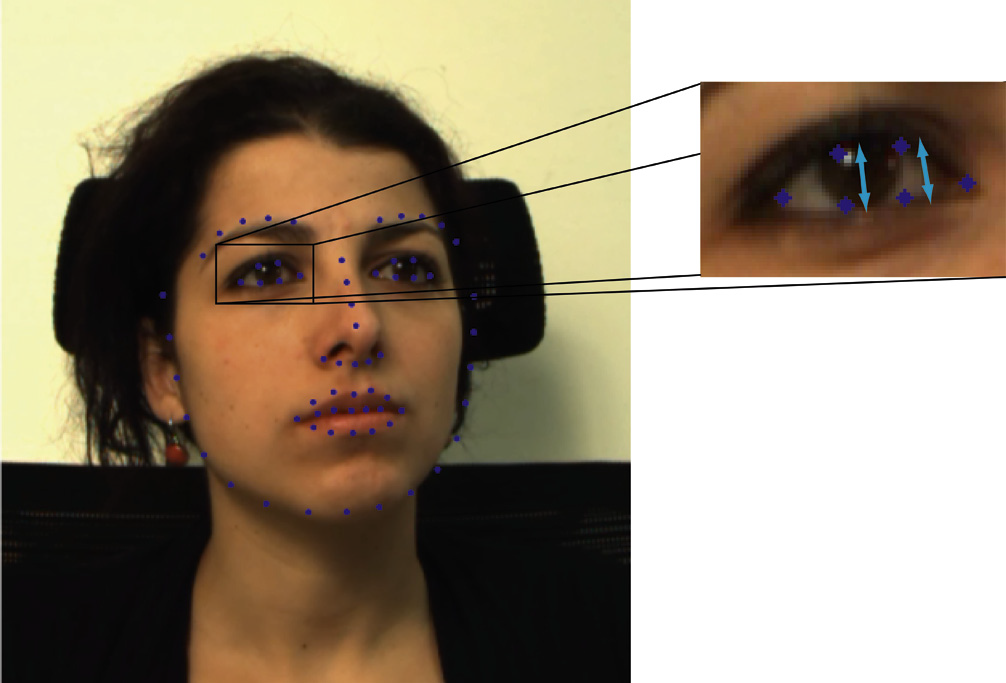
\includegraphics[width=\linewidth]{figures/giannakakis2017stress-eye.png}
    \caption{Highlight of average distance calculation regarding eye apperture \parencite{giannakakis2017stress}.}
    \label{fig:distance-samara}
\end{figure}
